\documentclass[conference]{IEEEtran}
\IEEEoverridecommandlockouts
% The preceding line is only needed to identify funding in the first footnote. If that is unneeded, please comment it out.
\usepackage{cite}
\usepackage{amsmath,amssymb,amsfonts}
\usepackage{algorithmic}
\usepackage{graphicx}
\usepackage{textcomp}
\usepackage{xcolor}
\usepackage{booktabs}
\usepackage{multirow}
\usepackage{colortbl}
\usepackage{float}
\def\BibTeX{{\rm B\kern-.05em{\sc i\kern-.025em b}\kern-.08em
    T\kern-.1667em\lower.7ex\hbox{E}\kern-.125emX}}

\bibliographystyle{IEEEtran}


\begin{document}

\title{Modelling Demographics using Monthly Electricity Consumption Data\\
% {\footnotesize \textsuperscript{*}Note: Sub-titles are not captured in Xplore and
% should not be used}

}

\author{\IEEEauthorblockN{Abdur Rahman}
\IEEEauthorblockA{\textit{School of Science and Engineering} \\
\textit{LUMS}\\
Lahore, Pakistan \\
email address or ORCID}
\and
\IEEEauthorblockN{Ameera Arif}
\IEEEauthorblockA{\textit{School of Science and Engineering} \\
\textit{LUMS}\\
Lahore, Pakistan \\
email address or ORCID}
\and
\IEEEauthorblockN{Ahmad Nadeem}
\IEEEauthorblockA{\textit{School of Science and Engineering} \\
\textit{LUMS}\\
Lahore, Pakistan \\
email address or ORCID}
\and
\IEEEauthorblockN{Naveed Arshad}
\IEEEauthorblockA{\textit{School of Science and Engineering} \\
\textit{LUMS}\\
Lahore, Pakistan \\
email address or ORCID}
}

\maketitle

\begin{abstract}
Electricity is one of the most widely used and exigent form of energy where human life has directly or indirectly become extensively dependent on it. It is becoming highly tedious for the energy sector to manage the modern consumer demands based on the constantly changing consumer demographics. It has therefore, become pertinent for the utility companies to evolve their development plans, tariffs and business models according to the consumer requirements. This article presents three different models multiple linear regression (MLR), support vector regression (SVR) and artificial neural network (ANN) to predict the attributes of a consumer household. The proposed technique uses the readily available monthly electricity consumption data. PRECON dataset is used to train and test the developed models. After performing extensive data cleaning and transformation we have selected six of the most relevant attributes available in the PRECON metadata to be predicted. 

ADD QUANTITATIVE RESULTS

\end{abstract}

\begin{IEEEkeywords}
energy prediction, residential building, machine learning algorithm, electricity consumption, demographics, consumer profile
\end{IEEEkeywords}



\section{Introduction}
Energy is integral to both life and its ability to perpetuate. A contemporary human life, marked by an amplified dependence on profuse, technologically oriented and advanced energy resources calls for newer, sustainable and more sophisticated models of energy distribution. The efforts toward unearthing and utilizing sustainable energy sources to meet the modern energy requisites are not only paramount in sanctioning a sustainable and secure future for this planet but also play a vital role in the current social and economic capability and development. In this context, electricity is one of the most widely used and exigent form of energy where human life has directly or indirectly become extensively dependent on it. It is predominantly generated through conventional power sources such as fossil fuels, nuclear power and hydro power and unconventionally through solar power and several renewable sources of energy. The generated energy is then supplied to the consumers by the power grids and distribution companies at fixed rates. It is becoming highly tedious for the energy sector to manage the modern consumer demands based on the constantly changing consumer demographic. According to the Pakistan Economic Survey 2019–20, electrical power consumption per capita has increased by 23.5\% \cite{data} over the period of 2000 to 2020. It has therefore, become pertinent for the distribution companies (DISCOs) to handle the distribution load according to the changes and patterns of the consumer’s electricity demand.  

In order for the energy sector of Pakistan to develop in a sustainable way, the DISCOs need to effectively start incorporating the consumer demographics and consumer-driven approach for future. The demographics and the consumption patterns of the consumers can prove to be a significant source of relevant insights needed for long term planning of energy optimization. The data extracted shall help the distribution companies to manage the revenue assessments, unit maintenance, scheduling, energy trading, expansion planning and to improve energy efficiency. Most importantly, the data can and will allow the companies to develop an optimal generation schedule to address the demand accordingly. In addition, policy makers will also be able to review the current strategies to minimize the electricity supply and demand gap and develop future strategies that will ensure affordable electricity with efficient generation, transmission and distribution though out Pakistan. 


The sufficient and accurate supply, availability and collection of the relevant data is one of the biggest hurdles in this process. The most typical methods of consumer demographics data collection include surveys, census, or simulations which are highly flawed, inefficient and very uneconomical. Another study offers the country-wide installation of smart meters as an alternate solution. When the idea was initially pitched in the early 2020, a capital expenditure of at least \$6 billion was estimated to cover the 90\% of a 35 million electricity consumer base \cite{theexpresstribune_2020}. However, in comparison, a total cost of only \$1.3 billion was invested in New York to employ 4.7 million meters to its gas and electric customers \cite{tweed_2015}. Unfortunately, such huge figures are hindering the progress of the plan even before its start. Considering the economic condition of especially the developing countries, such as Pakistan, with meagre resources and none to spare, such resource hungry methods are not practicable. The proposed technique in this paper uses the readily available monthly electricity consumption data to predict the consumer demographics, which is much more pragmatic. This technique can serve as a blueprint for other developing countries as well.


To this end, this research proposes a novel consumer demographic prediction model from monthly electricity consumption data and evaluates its performance using mean absolute percentage error metric. This research has been successful in achieving state-of-the-art accuracy in the model by applying data refinement techniques, followed by data training using three different machine learning algorithms.

The rest of the paper is organized as follows. Section II discusses the work previously done in this domain. Section III analyzes the characteristics of the data and proposes 3 different techniques. Implementation of forecasting techniques and results are discussed in Section IV. Finally, conclusions are drawn in Section V. 



\section{Literature Review}
It is pivotal to understand the role of energy sector and more specifically electricity in the economic development, technological advancement, and planning of a country. To monitor household power consumption non-intrusive load monitoring is used which not only gives an analysis of the consumer behavior but also explores energy conservation patterns. Biansoongnern,S. et al. present an NLIM (non-intrusive load monitoring) model in \cite{BIANSOONGNERN2016172} which measures the electricity consumption of some particular appliances without installing additional instruments which reduces cost and time and achieves significant saving in energy consumption by using real time information. In another paper Berges, M. et al, discuss an NLIM approach that can give feedback about the energy consumed in a residential building along with the operational schedule of appliances \cite{articleBerges}. Some NLIM methods use the steady state operations of the appliances for energy disaggregation. In \cite{5582070},
the writers use steady state energy used pattern to classify cases of step change by measuring energy usage at circuit level. But a problem in this is that it gives poor performance in recognizing particular load types. Besides analyzing the load patterns it is imperative that the consumption as well as the demand patterns for electricity are forecasted to counter the present and future needs. Huge amount of research has been done in this respect ranging from different forecasting models and techniques to economic indicators and electric loads on all horizons (i.e., short, medium and long terms). 

% ARIMA, one of the initial models for time series forecasting is used by Kaur, H. and   Ahuja, S. \cite{kaur_ahuja_2017} to predict electricity consumption of a health care institution in terms of monthly, bimonthly, or quarterly time series. In \cite{Theile2018DayaheadEC}, P. Theile et al. focus on predicting power consumption using two machine learning algorithms, Support Vector Machine (SVM) and Recurrent Neural Network (RNN) which are highly accurate in predicting day-ahead half-hourly power consumption data along with providing useful insights on data handling. 
A model is proposed \cite{bot_ruano_ruano_2020} where household electricity consumption is forecasted using support vector regression. One of the most significant contributions to the present research and literature on load forecasting is related to the variable selection approach used in determining the best subset of consumption predictors used. It selects 18 of the 48 initial variables as the critical predictors. As the nature of algorithms progressed and a new era of artificial intelligence started, Singh, S. et.al's study \cite{singh_hussain_bazaz_2017} proposed the use of ANN for load forecasting. Considering the different load profiles for weekends and weekdays, they use separate neural networks for each. As technology progressed into the deep learning era, Troung et.al \cite{app11052229} proposed the usage of deep neural network-based energy prediction algorithm for accurately forecasting the day-ahead hourly energy consumption profile of a residential building using occupancy rate as an input and that gives a coefficient of determination of 97.5\%. A hybrid approach that employs Convolution Neural Network (CNN) and Gated Recurrent Units (GRU) into a unified framework for accurate energy consumption prediction has also been proposed \cite{articleSajjad} which acts as an effective alternative to the previous models in terms of computational complexity as well prediction accuracy. Another recent paper by Theile, P. et al. \cite{Theile2018DayaheadEC} focuses on predicting power consumption using two machine learning algorithms namely Support Vector Machine(SVM) and Recurrent Neural Network (RNN). The model incorporates time, day of the week, and the week number within the year to yields different results when either one of them is used for prediction. The RNN proposed the most substantial results with a mean error of 3.5227\%, obtained using the features such as temperature, weekday, tempo, and holiday. The literature also provides a solution to the problem of limited data by using transfer learning techniques \cite{DBLP:journals/corr/abs-1906-02646}. Firstly, CNN is used to capture the intraday, daily, and weekly cyclostationary patterns, trends and seasonality in energy assets time series. Then, transfer learning strategy is applied on the CNN model results to yield significant improvements. 

All the present literature proves to be invaluable in comprehending the role, significance and use of time series techniques for forecasting electricity demand however all the research has been limited to load prediction based on specific demographics. While this an advantage for energy providers and utility companies but there is room for more open and unrestrained research. Predicting the demographics of people from their energy loads still requires a considerable amount of research. The prediction approach presented in this paper provides substantial contribution towards introducing newer methods of demographics prediction. The proposed approach has not yet been forwarded as of our knowledge.\par



\section{Methodology}

Understanding  the  consumer demographics can transform the distribution networks and planning sector to a more effective and a consumer driven model. With the knowledge of consumer profiles, distribution companies can understand their customers better and thus introduce better plans and packages for all the different types of customers. Hence these DISCOs can expand their current business keeping in view the trend of overall consumer growth. Additionally, the high rate of transmission and distribution network failures, power theft and the load shedding is a huge problem in developing countries such as Pakistan \cite{articleHussain}. By understanding the electricity consumer's requirements and usage patterns, the DISCOs can identify such electricity loss cases \cite{articleJaiswal}. Lastly they can also introduce economical customized tariff packages for various different types of customers. Gaining the knowledge of the demographic parameters such number of ACs, fans and refrigerators will allow the DISCOs to better handle the degrading power factor and overloading of local distribution network in summer. Overall, a detailed knowledge on household level will make room for better regulation of customers and personalized services.


\subsection{Dataset}

For this study, Pakistan Residential Electricity Consumption (PRECON) dataset is used. It contains electricity consumption for a year (June 2018 to May 2019) for 42 residential properties having diverse demographics \cite{9194176}. The dataset can be regarded as a representative of electricity consumption profiles of residential buildings in South Asia. It is one of the pioneer datasets which covers such a vast scale of information. It covers consumption patters from all aspects ranging from different house sizes, to different number of electronic devices, and even incorporates permanent, temporary residents. The selected residential properties are scattered all over the city, which enabled to cover various types of households, varying in financial status, daily activities and usage pattern of home appliances.

The dataset contains some households with partly missing electricity consumption data. Therefore, these households are not suitable to be used in either training or testing of the machine learning models. After removing houses with missing data, 34 households are left. All the work described below uses data related to these filtered households. Out of all the attributed presented in PRECON, the following six are selected:

 \begin{itemize}
     \item Number of people
     \item Number of fans
     \item Number of air conditioners
     \item Number of refrigerators
     \item Property area
     \item Total number of rooms
 \end{itemize}
 
 The reason for selecting the aforementioned attributes it their significance for the distribution companies. Knowing the number of people, area of the property and information about other major home appliances will help DISCOs better manage the power system. For instance, having the knowledge of the number of installed air conditioners, fans and refrigerators can help DISCOs predict and mange the degrading power factor in summer. Having the knowledge of number of people can also help in prediction of short term residential load. These demographics can help system operator predict daily load patterns and their weekly and seasonal variation. Having the knowledge of property area can help the distribution company manage resources such as meter reading officials that traverse their allocated regions to gather electricity consumption data, since, due to lack of smart meters in developing countries, hiring meter reading officials is the most viable method.

Figure \ref{fig:metadata divers} shows the distribution of the selected attributes of the houses from the PRECON dataset. The box plot of number of people shows that the median number of people living in a house is 6 and it goes as high as 10 with one outlier having 11 people. Similarly, the median number of installed air conditioners in a house is 4 which goes as high as 11. Overall, this dataset covers diverse demographics and is therefore suitable for training machine learning models. 


\begin{figure}[ht]
\centering{\includegraphics[width=85mm]{images/metadata diversity 2.png}}
\caption{Diversity in customer demographics data}
\label{fig:metadata divers}
\end{figure}

Figure \ref{fig:consumption distri} shows the distribution of monthly energy consumption calculated by aggregating PRECON data available originally at minute intervals. The length of the box plots shows the amount of variation in each month. In Pakistan, summer ranges from May till September which is reflected by higher electricity consumption in those months. Other than the summer months the residential electricity consumption remains low because of absence of cooling load such as air conditioners, fans and refrigerators. All this information will be helpful in training the models.



\begin{figure}[ht]
\centering{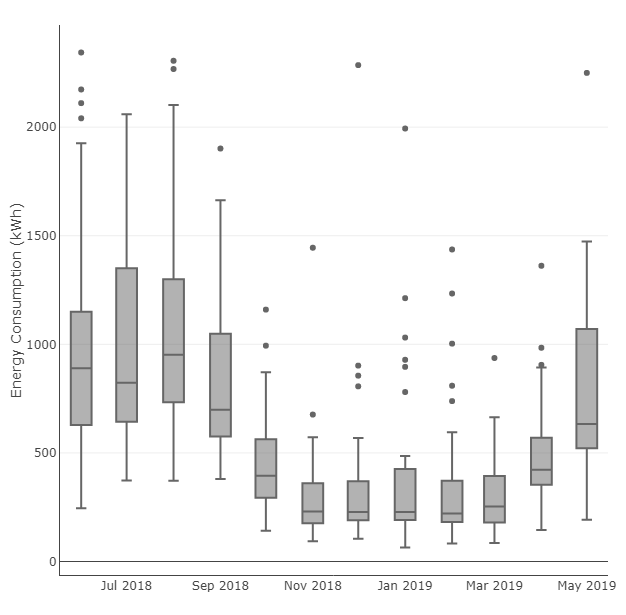
\includegraphics[width=85mm]{consumption distribution.png}}
\caption{Monthly electricity consumption distribution}
\label{fig:consumption distri}
\end{figure}


\subsection{Multivariate Linear Regression (MLR)}

To predict the six attributes described above, the first model used is multiple linear regression \cite{bottenberg1963applied}. Monthly electricity consumption for the whole year creates twelve independent input variables. These input variables are used to develop six equations for each of the six attributes. A generic form of the equation is given in \ref{eq:linearmodegeneric}.   

\begin{equation}
Y = \beta_0 + \sum_{i = 1}^{n}\beta_i X_i 
\label{eq:linearmodegeneric}
\end{equation}

where \(X_i\) is the electricity consumption for a month and \(Y\) is the predictor variable. \({\beta}_0\) is the intercept. \(n\) is the total number of months. \(B_i\) is the gradient coefficient of electricity consumption of each month. To achieve a better prediction, a minimum threshold for p-value was set and step-wise bi-directional selection \cite{wang2013comparison} was used to eliminate predictor variables. Gradient coefficients of independent variables rejected after stepwise selection are zero.


\subsection{Support Vector Regression (SVR)}
Support Vector Regression (SVR) is the second model in this study which uses the same principle as support vector machine, but it is modified for regression problems. It works by finding a hyper-plane in an N-dimensional space, where N is the number of features, to distinctly classify the data points \cite{drucker1997support}. Radial Basis Function (RBF) kernel has been used which models the non-linearity between the independent variables and the predictors. It allows the tuning of gamma and cost hyperparameters which controls the complexity and smoothing of the model.



\subsection{Artificial Neural Network (ANN)}
Neural networks have gained a great deal of popularity owing to their possibility in solving both classification and regression problems \cite{specht1991general}. We have used neural network for regression to predict the household demographics. The number of layers, number of neurons, activation functions, learning rates are tuned for each attribute to achieve the best accuracies. Initially, each node in a neural network is assigned a numerical weight randomly which is tuned through back propagation. These weights regulate the amplitude of the signal that passes between them. A sample of the neural networks used in this study is shown in the figure \ref{fig:nn for no of people}.


\begin{figure}[ht]
\centering{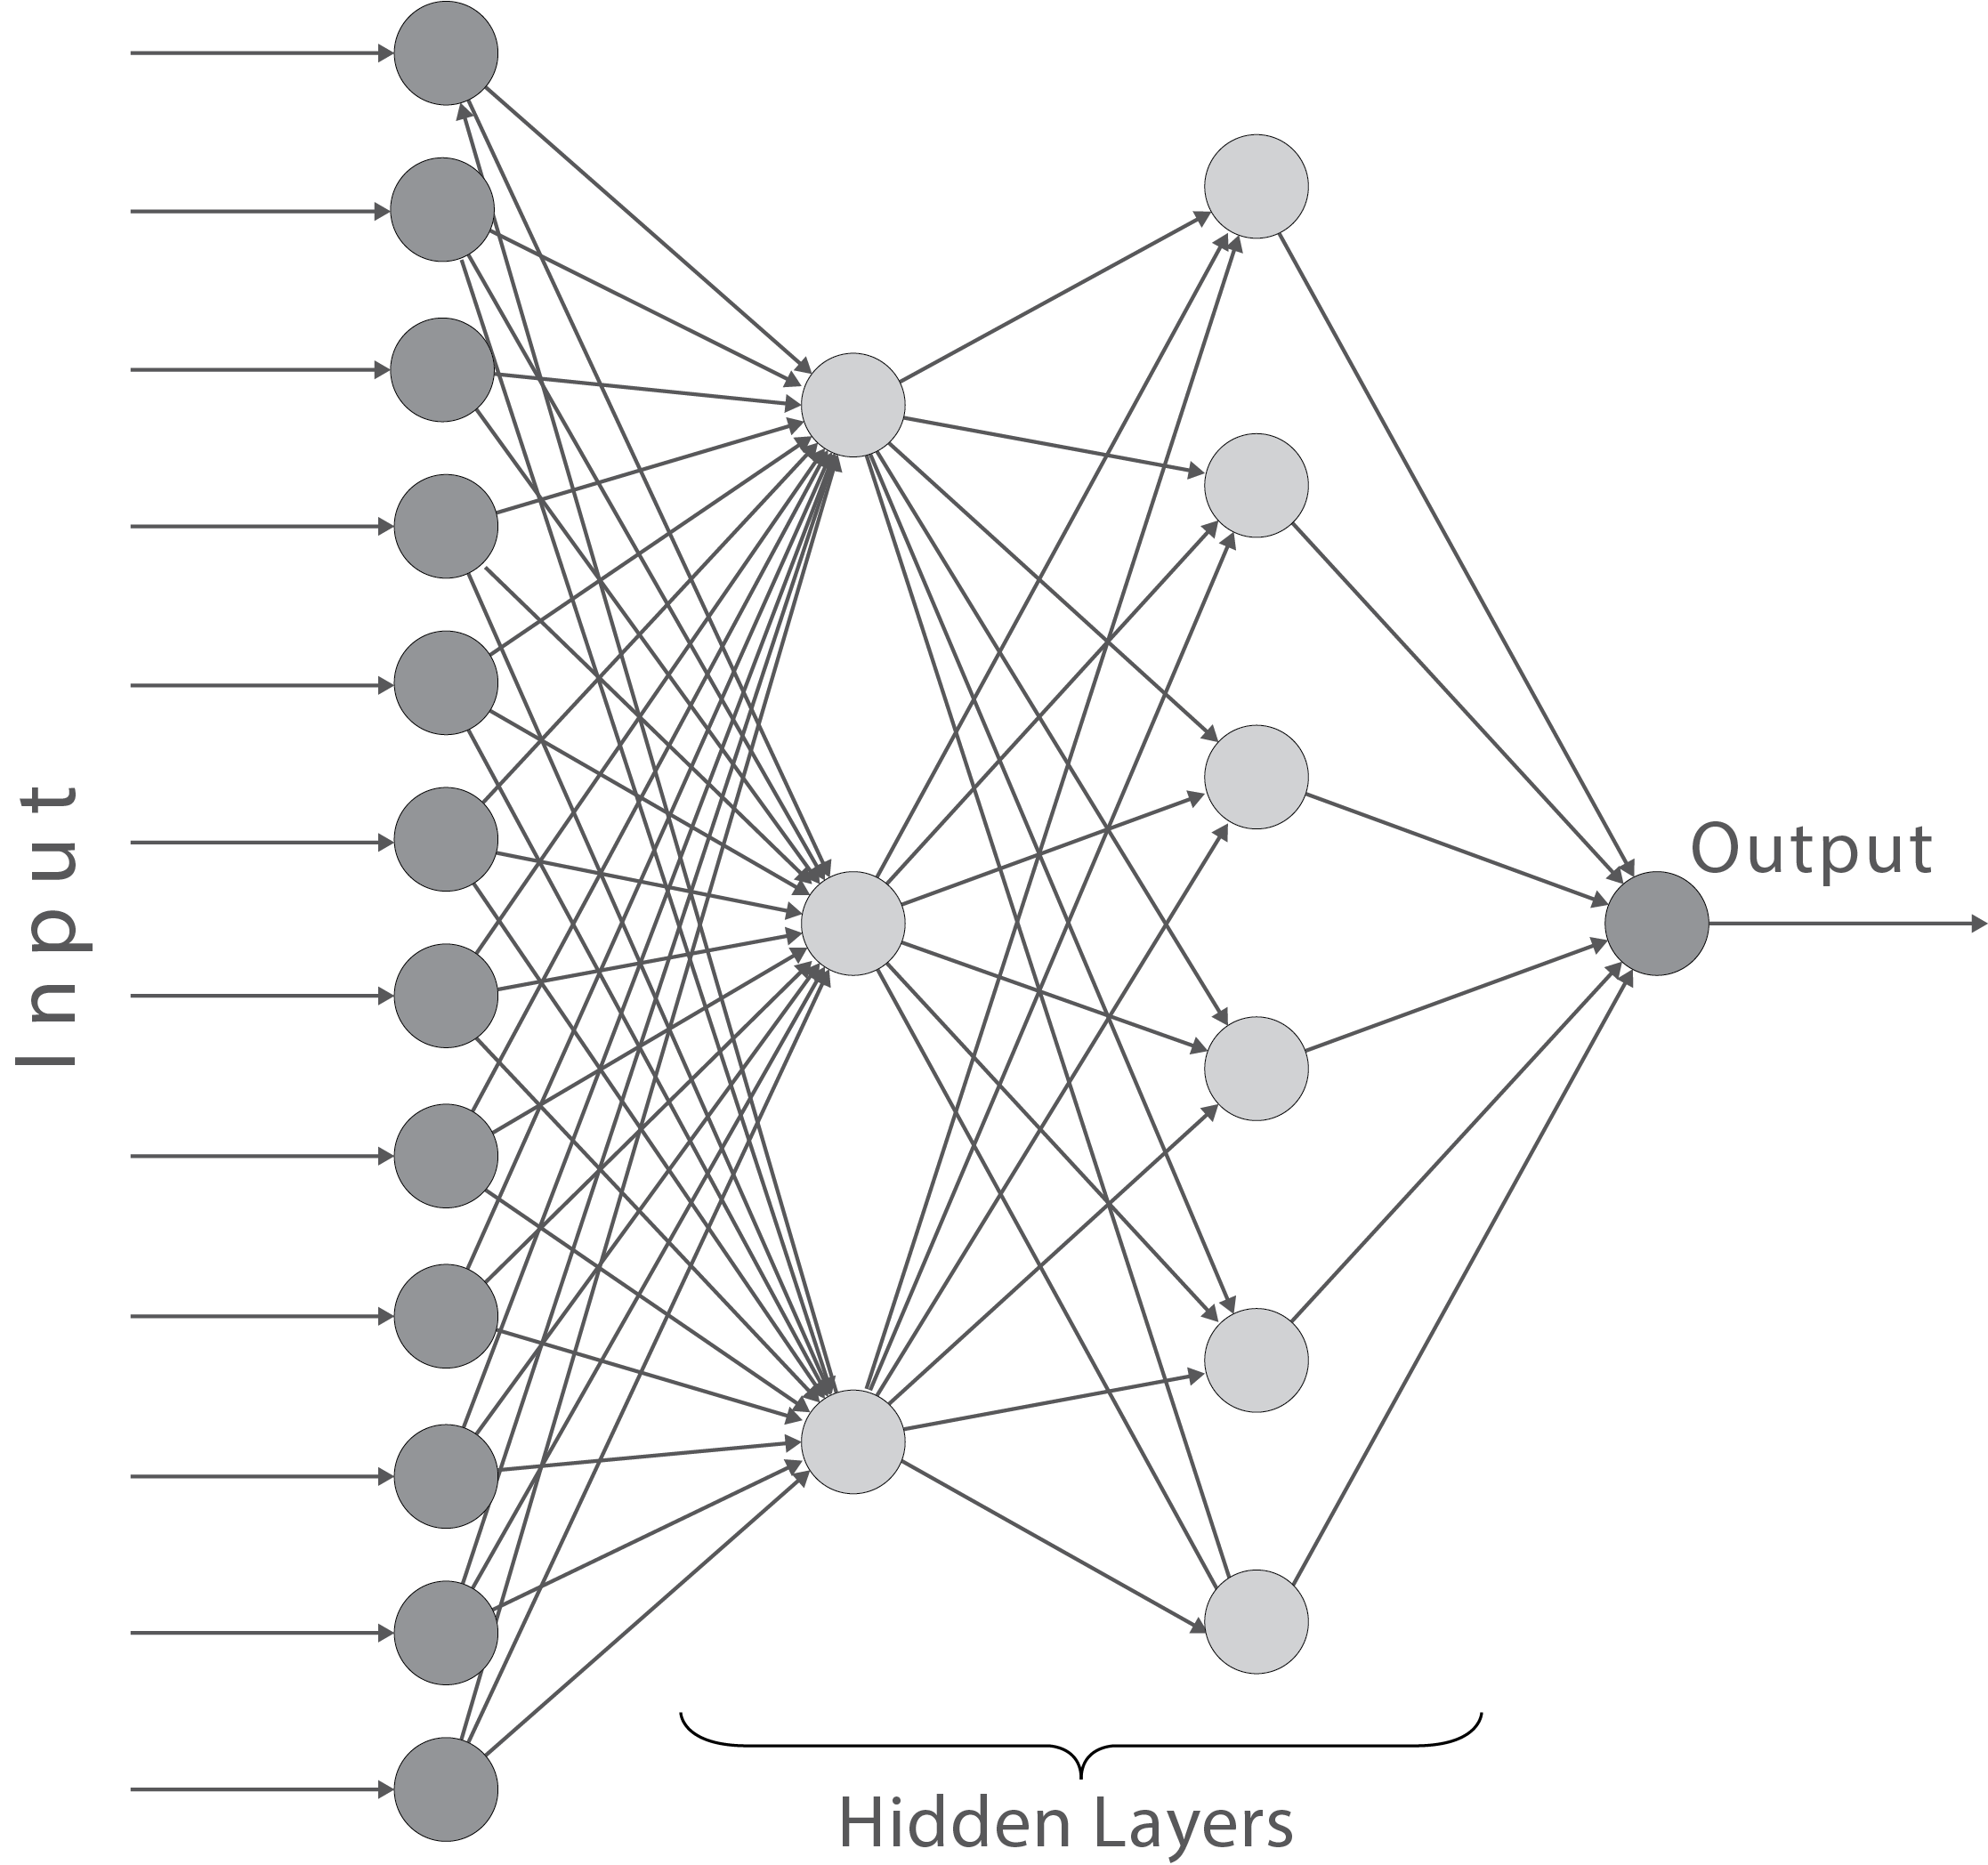
\includegraphics[width=85mm]{images/neural_net.png}}
\caption{Neural network for number of people}
\label{fig:nn for no of people}
\end{figure}


\subsection{Evaluation Criteria}
Various techniques are used to evaluate the performance of regression models. The commonly used error metrics are  Mean Error (ME), Mean Absolute Error (MAE) and Mean Absolute Percentage Error (MAPE). As ME takes the average of the difference between actual and predicted values it is prone to negation of over and under estimation by the model. Hence, it may create a false indication of better model performance. MAE addresses this problem by taking the absolute value of the calculated error, however, it does not depict the significance of that error with respect to the actual value. In this regard, MAPE covers both these issues and hence, is a better indicator for the evaluation and comparison of the three models used in this study. MAPE can be calculated using the fomula given in equation \ref{eq:mapeequation}.

\begin{equation}
    MAPE = \frac{1}{n}\sum_{t = 1}^{n}\displaystyle\left\lvert \frac{A_t - P_t}{A_t} \right\rvert
    \label{eq:mapeequation}
\end{equation}
where \(n\) is the number of test samples, \(A\) is the actual value and \(P\) is the value predicted by the model.




\section{Results and Discussion}

The selected households obtained after cleaning and pre-processing of the data, are divided into train and test subsets with 30 and 4 households respectively. The models are trained using the parameters mentioned above and the finalized models are used for predicting the test subset. The performance of each model is then evaluated using MAPE as shown in table \ref{table: tablemape}.  

The table \ref{table: tablebetacoeffs} shows the intercept and the gradient coefficients calculated from multiple linear regression models. To predict property area using MLR, electricity consumption of July, November and December 2018 is used with gradient coefficients of -5.28, 18.98 and 5.6 respectively. All three of the independent variables used show significance in explaining the variance in property area, as for all, p-value is less than 5\%. Rest of the months are rejected by the stepwise bi-directional selection algorithm due to their p-value being higher than 10\%. Table \ref{table: tablebetacoeffs} also shows the accepted independent variables for the rest of the attributes as well as their p-values. 

All the three models play their role in predicting important consumer demographics. Linear model is able to predict the number of people with very low error relative to the other two models with MAPE of 3.57\% which is represented with a dark shaded cell in the table \ref{table: tablemape}. This is further complemented by table \ref{table: tablebetacoeffs} which shows that the number of people primarily holds a strong linear relationship with the consumption of the month of June 2018 and August 2018. For the month of June 2018, the number of people has a negative linear relation with the electricity consumption while it has a positive linear relation with electricity consumption of August 2018 with gradient coefficients of -0.002 and 0.004 respectively. The performance of all three models is not satisfactory for predicting property area with minimum MAPE of 141.31\% reported by SVR. This can be attributed to the limited dataset. Number of refrigerators were predicted by both linear regression and support vector regression with MAPE of 8.33\%, outperforming the neural network. For the number of fans, air conditioners and rooms, ANN was able to give much lower MAPE than the MLR and SVR.




\begin{table}[ht]
\centering
\caption{Mean absolute percentage error obtained from the three prediction models}
\setlength{\tabcolsep}{2pt}
\begin{tabular}{lccc}
  \toprule 
  \multirow{2}{*}{Parameter} & \multicolumn{3}{c}{MAPE}\\
  \cmidrule(l){2-4}
   & MLR & SVR & ANN\\ 
  \midrule
  Number of people & \cellcolor{gray!70}3.57 & \cellcolor{gray!30}21.07 & \cellcolor{gray!50}9.12 \\ 
  Number of fans & \cellcolor{gray!10}59.17 & \cellcolor{gray!10}65.00 & \cellcolor{gray!50}10.00\\
  Number of air conditioners & \cellcolor{gray!10}77.38 & \cellcolor{gray!10}66.07 & \cellcolor{gray!50}11.90 \\ 
  Number of rooms & \cellcolor{gray!10}44.04 & \cellcolor{gray!10}40.48 & \cellcolor{gray!50}10.71 \\ 
  Number of refrigerators & \cellcolor{gray!50}8.33 & \cellcolor{gray!50}8.33 & \cellcolor{gray!30}25.00 \\ 
  Property area (sqft) & \cellcolor{gray!10}226.90 & \cellcolor{gray!10}141.31 & \cellcolor{gray!10}189.80 \\ 
  \bottomrule
  \label{table: tablemape}
\end{tabular}
\end{table}


\begin{table*}[h]
\centering
\caption{Coefficient with their p-values in parenthesis obtained using MLR}
\begin{tabular}{lcccccccc}
  \hline
 & Property Area & Rooms & People & ACs & Refrigerators & Fans \\ 
  \hline
Intercept  & 2143.1(0.03) 	& 4.24(~0)     		& 3.94(~0)          & 2.2(~0)      	& 1.61(~0)  	& 5.36(~0)\\ 
  Jun 2018 & -      		& -			    	& -0.002(0.05)	    & -  			& -   			& -\\ 
  Jul 2018 & -5.28(~0) 		& -             	& -                 & -   			& -  			& -\\ 
  Aug 2018 & -			  	& -         		& 0.004(0.009)     	& - 			& -         	& - \\ 
  Sep 2018 & -      		& -         		& -                 & -     		& - 			& - \\ 
  Oct 2018 & -      		& -         		& -                 & -      		& -				& -\\ 
  Nov 2018 & 18.98(~0)  	& -         		& -                 & -  			& -     		& - \\ 
  Dec 2018 & 5.6(0.03)  	& -         		& -			     	& -			  	& -     		& -\\ 
  Jan 2019 & -			  	& -0.004(~0)   		& -			 		& -			  	& -     		& -\\ 
  Feb 2019 & -      		& -			    	& -                	& 0.006(~0) 	& -     		& -\\ 
  Mar 2019 & -  	    	& 0.014(~0)         & -                 & -     		& 0.004(0.03)	& 0.01(~0)\\ 
  Apr 2019 & - 	   	  		& -         		& -                 & -   			& -     		& - \\ 
  May 2019 & - 		     	& -				   	& -                 & -  			& -0.0015(0.04)	& - \\ 
   \hline
   \label{table: tablebetacoeffs}
\end{tabular}
\end{table*}


The results presented in this study provide satisfactory results for some attributes such as number of people and air conditioners. However, one of the important attribute, property area, is not explained well by any of the three models, as evident from the reported MAPE. This can be improved by expanding the dataset or by improving the models, tuning their various hyperparameters. Various other variants of MLR can be tested to achieve better results, using interactions between independent variables. In the same way, other kernels such as sigmoid and polynomial can be explored in future to improve performance for demographic attributes. In this study, the neural network employs resilient backpropagation with weight backtracking. Other algorithms such as semi-log regression can be applied to minimize error. 


\section{Conclusion}
The motivation of this paper is based on the idea that knowledge of consumer demographics can substantially transform the business model of electricity distribution companies. This can not only help the distribution companies understand the needs of their customers in a better way but also provide customized tariff rates and better plans and packages for all of their diverse consumer base. It can also potentially solve the prevalent power distribution problems especially in the developing countries. A resource efficient method to predict residential consumer demographics from monthly electricity consumption data is proposed in this paper. We suggest three different techniques - multiple linear regression, support vector regression and neural network. Results show that several parameters can be predicted with MAPE of less than 12\%. Number of people can be predicted with a MAPE of approximately 4\% while the prediction of property area shows MAPE in the order of hundreds. Further work can be done to improve the reliability of the models by using different hyper parameters and using a larger dataset. The study can further be extended to include commercial and industrial consumers, predicting their different assets and


\bibliography{mybibfile}




\vspace{12pt}

\end{document}
